\documentclass[DIV12,a4paper]{scrartcl}

\usepackage%[demo]%
{graphicx}
\usepackage[utf8]{inputenc}
\usepackage{listings}
\usepackage{caption}
\usepackage{subcaption}

\graphicspath{ {figures/} }

\newcommand{\defaultwidth}{.8\textwidth}
\newcommand{\halfwidth}{.4\textwidth}

\usepackage{color}

\title{Laboration 2:\\ ASUS Xtion Pro: Calibration, noise characterization and filtering\\{\small Sensors and Sensing}}
\author{Michael Flo{\ss}mann, Anders Wilkstr\"om}
\date{2015--12--07}

\begin{document}
\maketitle

\section{Introduction: Structured light cameras}
Structured light cameras are a low-cost option for depth measuring in three dimensional space. The cameras project a known light pattern to a scene and record the reflection of that light pattern. This recorded data is then used for triangulation.\par
For this lab, the ASUS Xtion Pro sensor was used as a structured light camera.
\section{Task and implementation}
The task at hand was to set up and calibrating the sensor, as well as to characterize the noise in the depth measurement and to set up filtering routines.
\subsection{Basic setup}
To set up the camera, the package \texttt{openni2} for ros-indigo was used. When launching the node \texttt{openni2.launch}, it publishes a wide range of topics from the camera.\par %TODO: Maybe list ALL the topics?
For this laboration, only the topics which publish a viewable image were of interest. This included two main topics:%TODO: Explain the opencv shit

\begin{itemize}
  \item \texttt{/camera/rgb/}\\
    This topic publishes data from the RGB camera on the ASUS Xtion Pro. The topic \texttt{/camera/rgb/raw} shows the unprocessed RGB image like a regular camera. A sample image from this topic is shown in figure \ref{fig:rgb-raw}. %TODO!
  \item \texttt{/camera/depth/}\\
    This topic publishes the depth data as a 2D-array of float variables containing the depth values in meters. A sample image from this topic is shown in figure \ref{fig:depth}.
  \item \texttt{/camera/depth\_registered}\\
    This topic combines the RGB and the depth image into a coloured point cloud. A visualization of this topic through the tool \texttt{rviz} is shown in figure %TODO
\end{itemize}

\begin{figure}
  \centering
  
\includegraphics[width=\defaultwidth]{TODO.png}
  \label{fig:rgb-raw}
  \caption{Output image of \texttt{/camera/rgb/raw}}
\end{figure}

\begin{figure}[!htbp]
  \centering
  
\includegraphics[width=\defaultwidth]{TODO.png}
  \caption{Output image of \texttt{/camera/depth/}}
  \label{fig:depth}
\end{figure}

\begin{figure}[!htbp]
  \centering
  
\includegraphics[width=\defaultwidth]{TODO.png}
  \caption{Screenshot of the vizualized pointcloud of \texttt{/camera/depth\_registered}}
  \label{fig:depth_registered}
\end{figure}

\subsection{Basic ROS node}
\label{sec:basic-ros}
After the basic setup, a ROS node template was used as a base to process the images and point clouds published. The received images are shown in figure \ref{fig:rgb-save} and figure \ref{fig:depth-save}.

\begin{figure}[!htbp]
  \centering
  
\includegraphics[width=\defaultwidth]{TODO.png}
  \caption{Save of the RGB image}
  \label{fig:rgb-save}
\end{figure}

\begin{figure}[!htbp]
  \centering
  
\includegraphics[width=\defaultwidth]{TODO.png}
  \caption{Save of the depth point cloud}
  \label{fig:depth-save}
\end{figure}

\subsection{Color camera calibration}
\label{sec:calibration}

\newpage
\subsection{Noise characterization}
\label{sec:noise_characterization}
%Modify your ROS node to observe a small window of depth image pixels around the center of the image.  Compute average and standard deviation distances for measurements within the window
In this part we cropped small windows of varying sizes in the center of the depth image. Then the camera was placed in several known distances from a wall and the average and standard deviation of the depth values in the cropped images were recorded.\par
The mean error of 10 seconds of measurement in relation to the distance is shown in figure \ref{fig:mean_error}. The variances are shown in figure \ref{fig:variance}.\par
\begin{figure}[!htbp]
  \centering
  \includegraphics[height=0.8\textwidth,angle=270]{figures/distance_values.eps}
  \caption{Mean absolute error of the mean depth in relation to the ground truth distance}
  \label{fig:mean_error}
\end{figure}
\begin{figure}[!htbp]
  \centering
  \includegraphics[height=0.8\textwidth,angle=270]{figures/variances.eps}
  \caption{Mean of the Variance of the depth in relation to the ground truth distance}
  \label{fig:variance}
\end{figure}
Analysing the mean error (fig. \ref{fig:mean_error}), no conclusive pattern can be recognized in relation of the window size and the ground truth distance. The variance (fig. \ref{fig:variance}) on the other hand increases with the distance and the window size. This can be explained by the geometric characteristics of the measurement (see fig.\ref{fig:geometric_representation}).
\begin{figure}[!ht]
  \centering
   %\input{figures/geometric_example.eps_tex}
  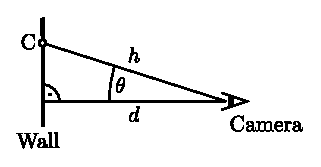
\includegraphics[width=.4\textwidth]{geometric_example.eps}
  \caption{Schematic of the distance measurement}
  \label{fig:geometric_representation}
\end{figure}\par
Figure \ref{fig:geometric_representation} shows a 2D schematic view of the measurement. The camera records the depth values of an area around a maximum value of $\theta$. The depth value at $C$ doesn't contain the actually desired distance to the wall $d$, but rather\[ h=\frac{d}{\cos\theta}.\]
As the distance to the wall $d$ increases, so does the absolute error between $h$ and $d$. Increasing the observed window size increases $\theta$, which has a similar effect.

\newpage
\subsection{Noise filtering}
\label{sec:filtering}
In this part we applied several filters to the depth images in order to remove the noise from the measurement data. These filters are:
\begin{itemize}
\item Gaussian blur
\item Median filter
\item Bilateral filter
\item Median over several image samples
\item Average over several image samples
\end{itemize}
The effect on the image data after the application of the filters will be discussed in the following.

% \subsubsection{NaN values}
% \label{sec:nan}
% Whenever the sensor can't evaluate the IR data, the according pixel in the depth image receives a \texttt{NaN} value as the depth value. This can be caused by an object standing too close to the sensor or by IR rays not reaching the sensor due to shadow casting, obstructing objects or scattering. Leaving these \texttt{NaN} values in the image data for processing would negatively influence the filters and thus should to be replaced.\par
% Two ways of replacing the \texttt{NaN} values were considered: 
% \begin{itemize}
% \item Replacing the \texttt{NaN} values with a depth-value of 0.
% \item Replacing the \texttt{NaN} values with the last valid pixel scanned.
% \end{itemize}
% We chose the first method, since the replaced pixels are still identifiable as invalid. Thus, less information is lost.

\subsubsection{Filter effects}
\label{sec:filter_effects}
\begin{figure}[!htbp]
  \centering
  \includegraphics[width=\defaultwidth]{depth_Original.png}
  \caption{Original depth image}
  \label{fig:original_depth}
\end{figure}

\paragraph{Gaussian blur}
The gaussian blur filter (fig. \ref{fig:gaussian_blur}) blurs the contours of the observed objects. Additionally, the pixels with \texttt{NaN} values reproduce and strongly disturb the algorithm. This can be explained as every kernel containing a \texttt{NaN} value gives every pixel in the whole kernel a \texttt{NaN} value. This also explains the ``blocky'' artifacts in areas which originally contained small \texttt{NaN} speckles.
\begin{figure}[!htbp]
  \centering
  \includegraphics[width=\defaultwidth]{depth_GaussianBlur.png}
  \caption{Gaussian blur}
  \label{fig:gaussian_blur}
\end{figure}

\paragraph{Median filter}
The median filter (fig. \ref{fig:median_depth}) doesn't show a big difference to the original image.
\begin{figure}[!htbp]
  \centering
  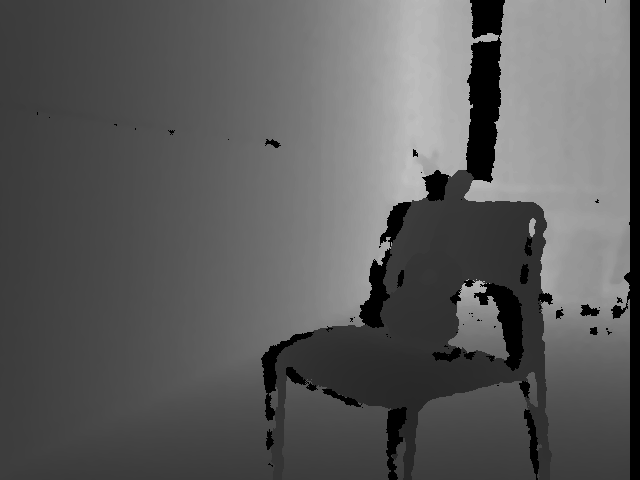
\includegraphics[width=\defaultwidth]{depth_medianBlur.png}
  \caption{Median filter}
  \label{fig:median_depth}
\end{figure}

\paragraph{Bilateral filter}
The bilateral filter (fig. \ref{fig:bilateral_depth}) blurs the contours of the objects. Otherwise, no remarkable differences to the original image are discernible.\par
In order for this filter not to produce very artifact-prone images, the \texttt{NaN}-values had to be adjusted. We chose to replace the \texttt{NaN}-values with entries of depth 0.
\begin{figure}[!htbp]
  \centering
  \includegraphics[width=\defaultwidth]{depth_bilateral.png}
  \caption{Bilateral filter}
  \label{fig:bilateral_depth}
\end{figure}
\paragraph{Median over several image samples}
The moving median image (fig. \ref{fig:moving_median_depth}) leaves the contours visible and removes smaller spots with \texttt{NaN} values.
\begin{figure}[!htbp]
  \centering
  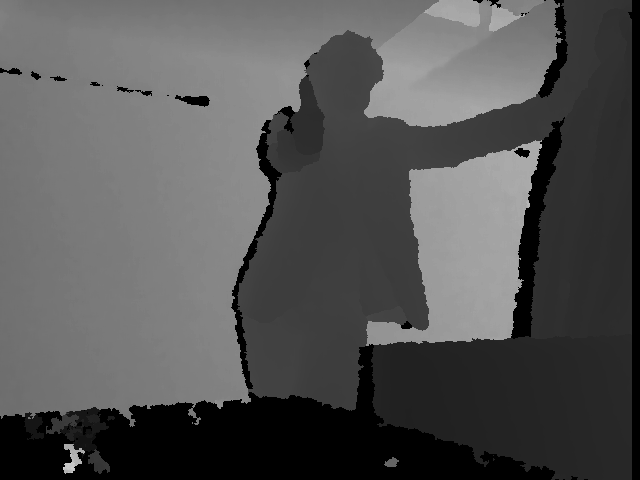
\includegraphics[width=\defaultwidth]{depth_MovingMedianFilter.png}
  \caption{Moving median image}
  \label{fig:moving_median_depth}
\end{figure}
\paragraph{Mean over several image samples}
The moving mean image (fig. \ref{fig:moving_mean_depth}) blurs the contours of the objects (although not as strongly as previous contour blurring algorithms). It also removes small speckles of \texttt{NaN} values.
\begin{figure}[!htbp]
  \centering
  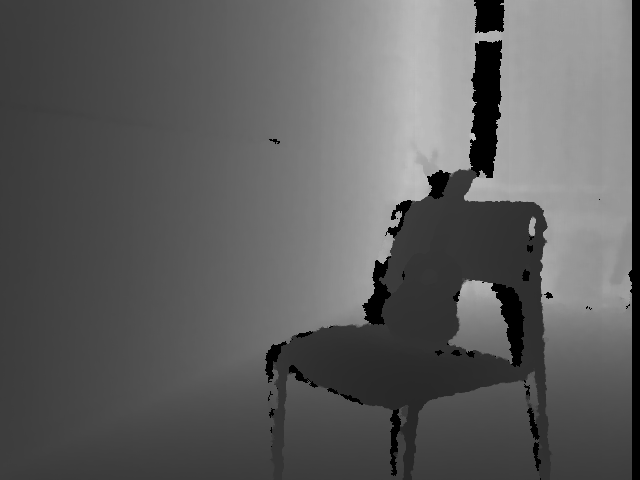
\includegraphics[width=\defaultwidth]{depth_MovingMeanFilter.png}
  \caption{Moving mean image}
  \label{fig:moving_mean_depth}
\end{figure}
\subsubsection{Salt-and-pepper removal properties}
\label{sec:grain_removal}
The depth images didn't suffer from noise clearly visible to the eye. In order to test the noise cancelling properties of the filters, artificial salt-and-pepper noise was added to the image file. This was achieved by changing random pixels in the image to black or white in each received depth-image. %TODO:Listing?
\par
\begin{figure}[!htbp]
  \centering
  \includegraphics[width=\defaultwidth]{depth_Original_spice.png}
  \caption{Original depth image with salt and pepper}
  \label{fig:original_depth_spice}
\end{figure}
\paragraph{Gaussian blur}
The gaussian blur (fig. \ref{fig:gaussian_blur_spice}) doesn't filter out the salt and pepper appropriately. It rather spreads the noisy data, negatively influencing the surrounding, proper data.
\begin{figure}[!htbp]
  \centering
  \includegraphics[width=\defaultwidth]{depth_GaussianBlur_spice.png}
  \caption{Gaussian blur with salt and pepper}
  \label{fig:gaussian_blur_spice}
\end{figure}
\paragraph{Median filter}
The median filter (fig. \ref{fig:median_depth_spice}) removes the salt and pepper speckles reliably.
\begin{figure}[!htbp]
  \centering
  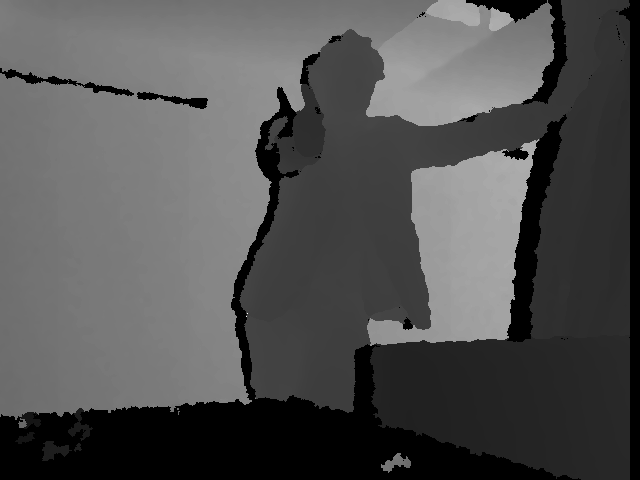
\includegraphics[width=\defaultwidth]{depth_medianBlur_spice.png}
  \caption{Median filter with salt and pepper}
  \label{fig:median_depth_spice}
\end{figure}
\paragraph{Bilateral filter}
The bilateral filter (fig. \ref{fig:bilateral_depth_spice}) decreases the influence of the salt and pepper speckles in the image, although they are still visible.
\begin{figure}[!htbp]
  \centering
  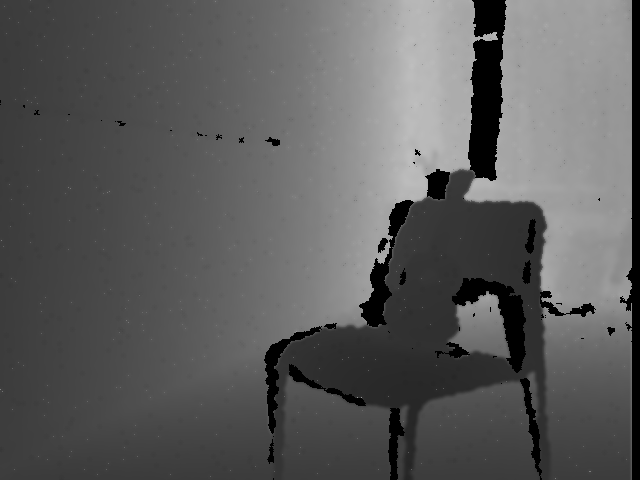
\includegraphics[width=\defaultwidth]{depth_bilateral_spice.png}
  \caption{Bilateral filter with salt and pepper}
  \label{fig:bilateral_depth_spice}
\end{figure}
\paragraph{Median over several image samples}
The bilateral filter (fig. \ref{fig:moving_median_depth_spice}) removes the salt and pepper speckles reliably.
\begin{figure}[!htbp]
  \centering
  \includegraphics[width=\defaultwidth]{depth_MovingMedianFilter_spice.png}
  \caption{Moving median image with salt and pepper}
  \label{fig:moving_median_depth_spice}
\end{figure}
\paragraph{Average over several image samples}
The bilateral filter (fig. \ref{fig:moving_mean_depth_spice}) accumulates the salt and pepper speckles of all recorded images. Although the speckles overall are more dull, their amount increased, still showing a considerable amount of noise.
\begin{figure}[!htbp]
  \centering
  \includegraphics[width=\defaultwidth]{depth_MovingMeanFilter_spice.png}
  \caption{Moving mean image with salt and pepper}
  \label{fig:moving_mean_depth_spice}
\end{figure}




\end{document}
